\chapter{Organisation et structure}

\section{Organisation du sujet}
L'organisation du projet a été soumit a un ordre de priorité car, comme cité dans "Mise en place du projet" (voir section \ref{sec:MEPprog}), certaines parties étaient nécessaires pour que d'autres fonctionnent ou puissent être amorcées :
\begin{itemize}
    \item En premier lieu nous fallait créer l'alphabet de notre L-Système (voir section \ref{sec:Alphabet}).
    \item Mise en place de méthode Parser\#isCorrect() pour vérifier certains que la syntaxe du l-système est correcte.
    \item Mise en place d'un moteur de réécriture.
    \item Mis en place d'un parser qui transforme le mot obtenu par le moteur de réécriture en une structure de données plus facilement lisible afin d'être afficher par le moteur graphique.
    \item affichage du L-Système dans le moteur graphique
\end{itemize}

\section{Structure du projet}
\begin{itemize}
    \item engine
    \begin{itemize}
        \item Rewrite: Moteur de réécriture
        \item Element, ElementProperties et Parser: voir section \ref{sec:parser}
    \end{itemize}
    \item screen
    \begin{itemize}
        \item gl3d: Tout les objets relatifs a l'affichage 3d du L-Systeme, voir la section \ref{sec:interface3d}
        \item main: Tout les objets relatifs au menu, voir la section \ref{sec:menu}
    \end{itemize}
    \item utils: contient l'objet Pair qui est essentiel au fonctionnement du projet
\end{itemize}

\begin{figure}[h!]
    \centering
    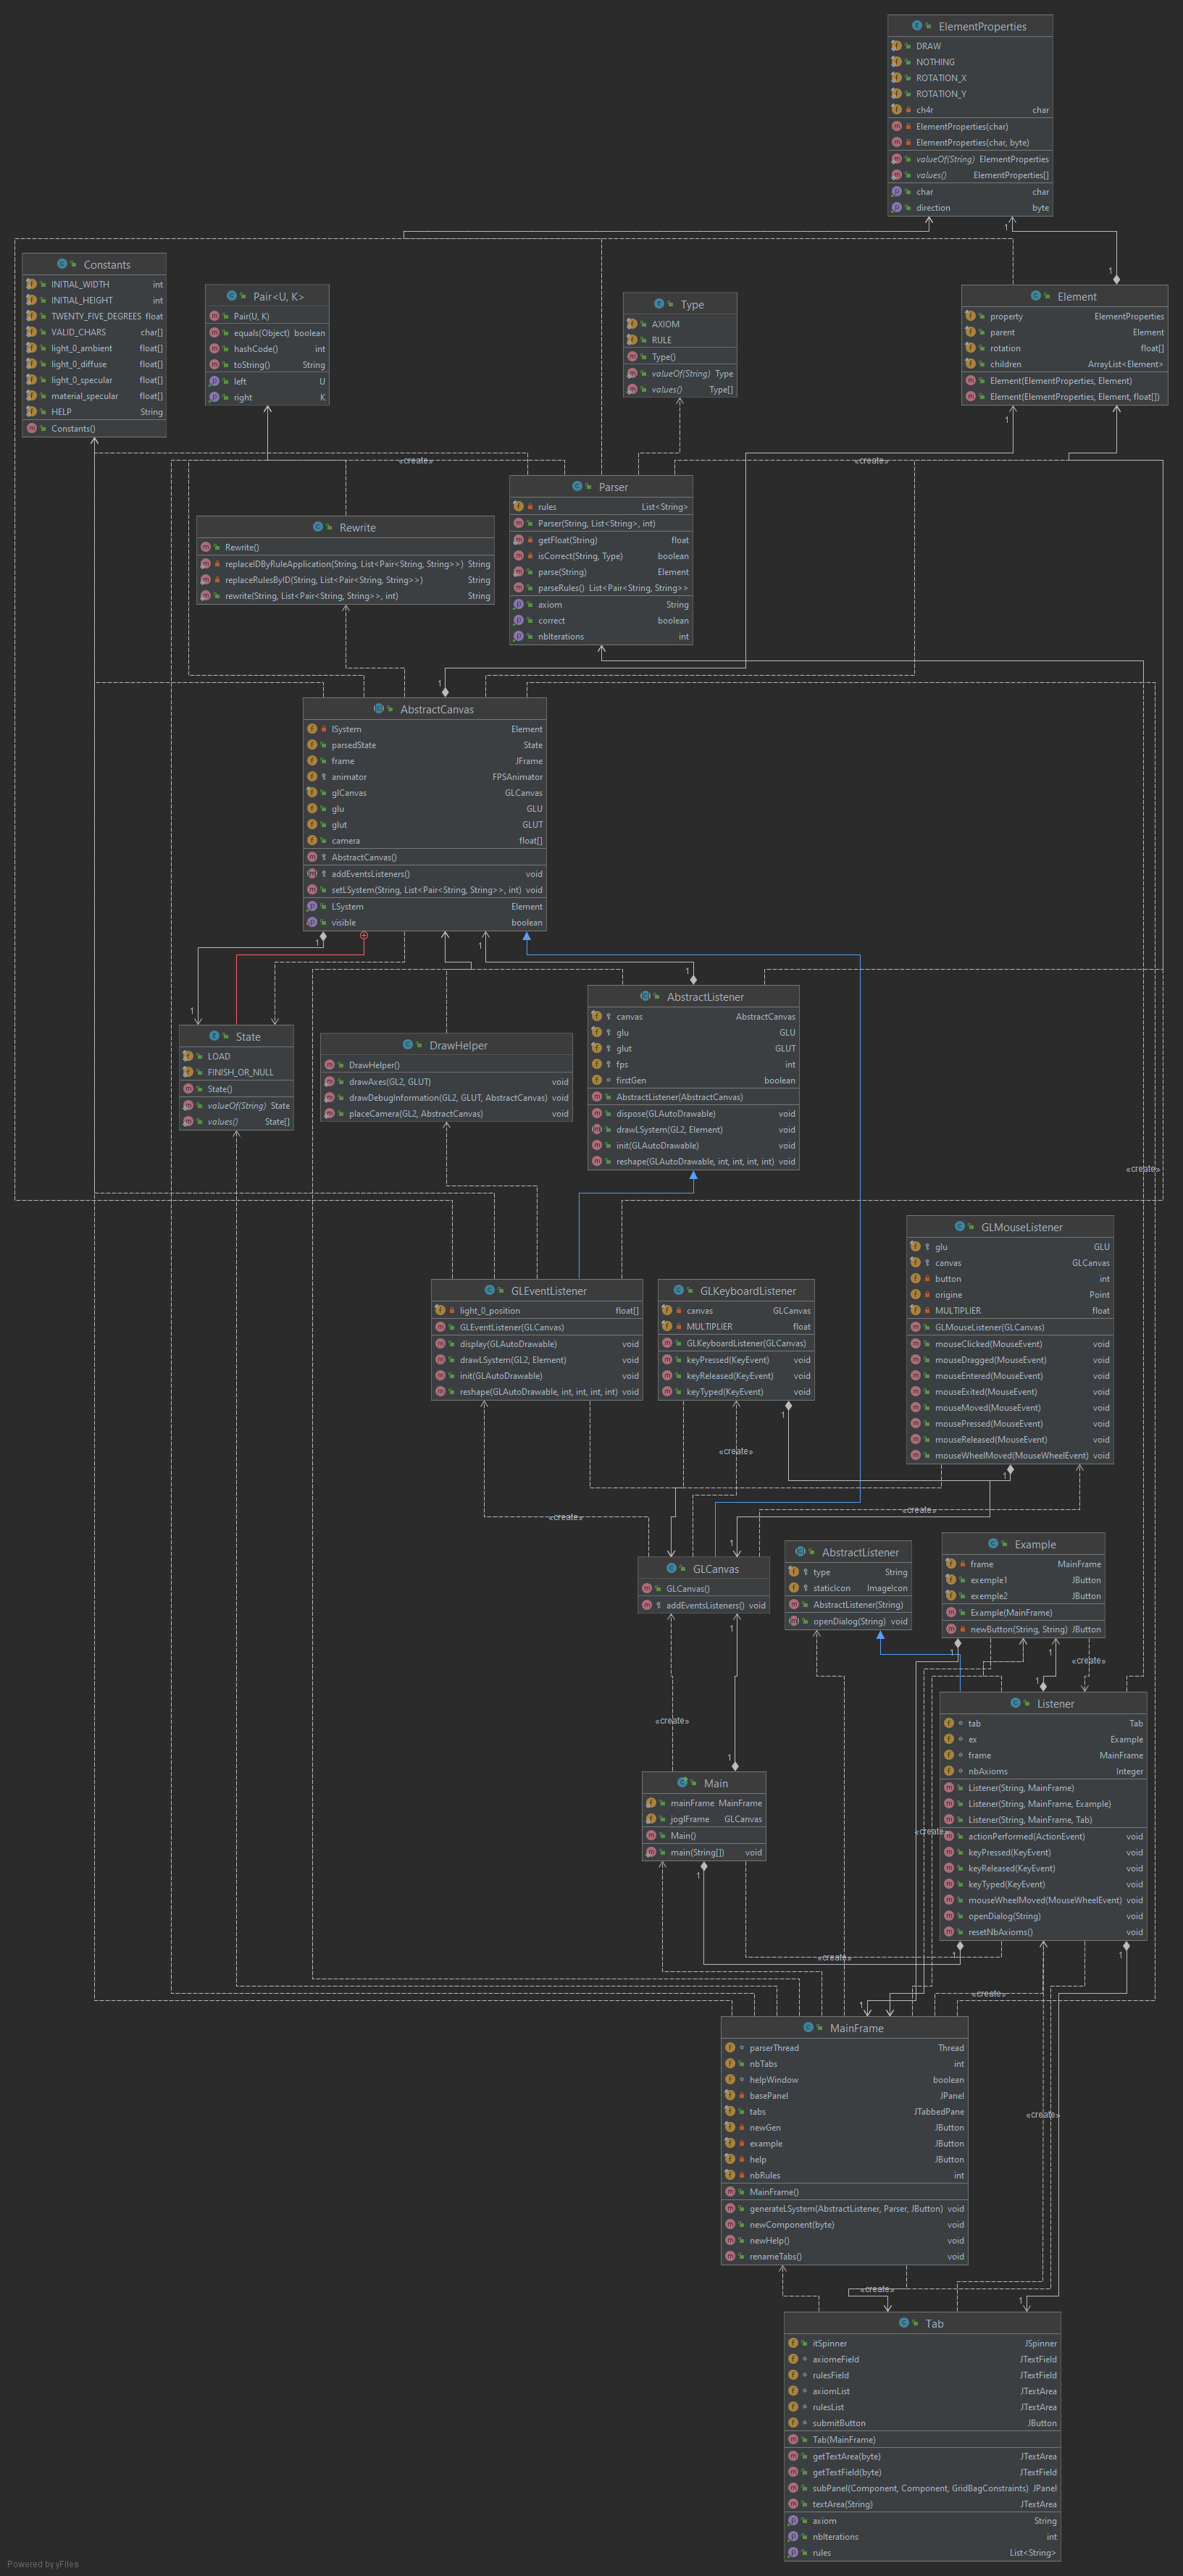
\includegraphics[width=0.7\linewidth]{pics/diagram.png}
    \caption{Diagramme de classe de notre projet}
    \label{fig:class_diagram}
\end{figure}

